%%%%%%%%%%%%%%%%%%%%%%%%%%%%%%%%%%%%%%%%%%%%%%%%%%%%%%%%%%%%%%%%%%%%%%%%%%%%%%%%%%
\begin{frame}[fragile]\frametitle{}
\begin{center}
{\Large Implementation using Microsoft Graph RAG}

{\footnotesize Source: Microsoft Research (https://microsoft.github.io/graphrag/) and GitHub repository (https://github.com/microsoft/graphrag)}
\end{center}
\end{frame}


%%%%%%%%%%%%%%%%%%%%%%%%%%%%%%%%%%%%%%%%%%%%%%%%%%%%%%%%%%%
\begin{frame}[fragile]\frametitle{Introduction to Microsoft's GraphRAG}
	\begin{itemize}
	\item GraphRAG is Microsoft's framework for RAG (Retrieval-Augmented Generation) on graphs
	\item Combines knowledge graphs with LLMs for enhanced context-aware responses
	\item Addresses limitations of traditional RAG by leveraging graph relationships
	\item Provides more structured, accurate, and explainable answers
    \item Open-sourced by Microsoft; code is available on GitHub.
    \item Works with both proprietary (e.g., GPT-4) and local models (e.g., LLaMA3).
    \item Aim: overcome limitations of traditional RAG systems.	
	\end{itemize}
\end{frame}

%%%%%%%%%%%%%%%%%%%%%%%%%%%%%%%%%%%%%%%%%%%%%%%%%%%%%%%%%%%
\begin{frame}[fragile]\frametitle{Traditional RAG Overview}
  \begin{itemize}
    \item Converts documents into vector embeddings via chunking.
    \item Stores chunks in a vector database.
    \item At query time: compute query embedding, retrieve similar chunks.
    \item Combines query + retrieved chunks to generate final answer.
  \end{itemize}
\end{frame}

%%%%%%%%%%%%%%%%%%%%%%%%%%%%%%%%%%%%%%%%%%%%%%%%%%%%%%%%%%%
\begin{frame}[fragile]\frametitle{Limitations of Traditional RAG}
  \begin{itemize}
    \item Lacks holistic understanding of entire document set.
    \item Retrieval efficiency drops as data size increases.
    \item Complex integration of external knowledge sources.
  \end{itemize}
\end{frame}

% %%%%%%%%%%%%%%%%%%%%%%%%%%%%%%%%%%%%%%%%%%%%%%%%%%%%%%%%%%%
% \begin{frame}[fragile]\frametitle{Traditional RAG: High-Level Flow}

	% \begin{center}
	% 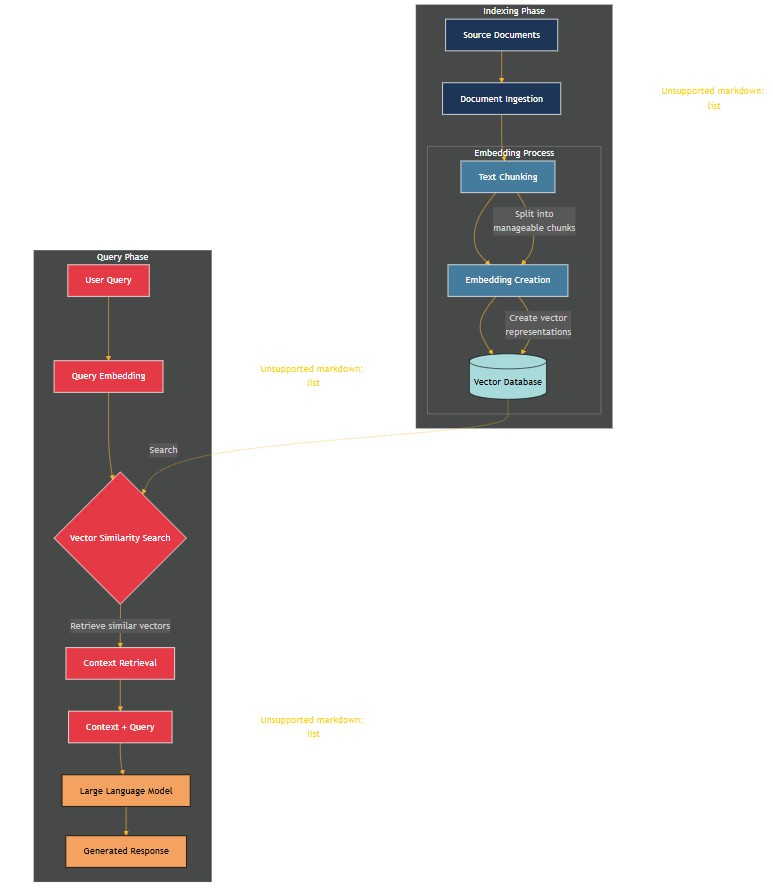
\includegraphics[width=0.5\linewidth,keepaspectratio]{graphrag_ms_2}
	% \end{center}
	
	% {\tiny (Ref: Graph RAG: Improving RAG with Knowledge Graphs: Prompt Engineering)}

	
% \end{frame}

%%%%%%%%%%%%%%%%%%%%%%%%%%%%%%%%%%%%%%%%%%%%%%%%%%%%%%%%%%%
\begin{frame}[fragile]\frametitle{GraphRAG: High-Level Flow}
  \begin{itemize}
    \item Two phases: indexing and querying.
    \item Entities and relationships extracted during indexing.
    \item Builds a knowledge graph, then forms communities of related entities.
    \item Summaries are generated at different levels of detail.
  \end{itemize}
\end{frame}

%%%%%%%%%%%%%%%%%%%%%%%%%%%%%%%%%%%%%%%%%%%%%%%%%%%%%%%%%%%
\begin{frame}[fragile]\frametitle{GraphRAG: High-Level Flow}

	\begin{center}
	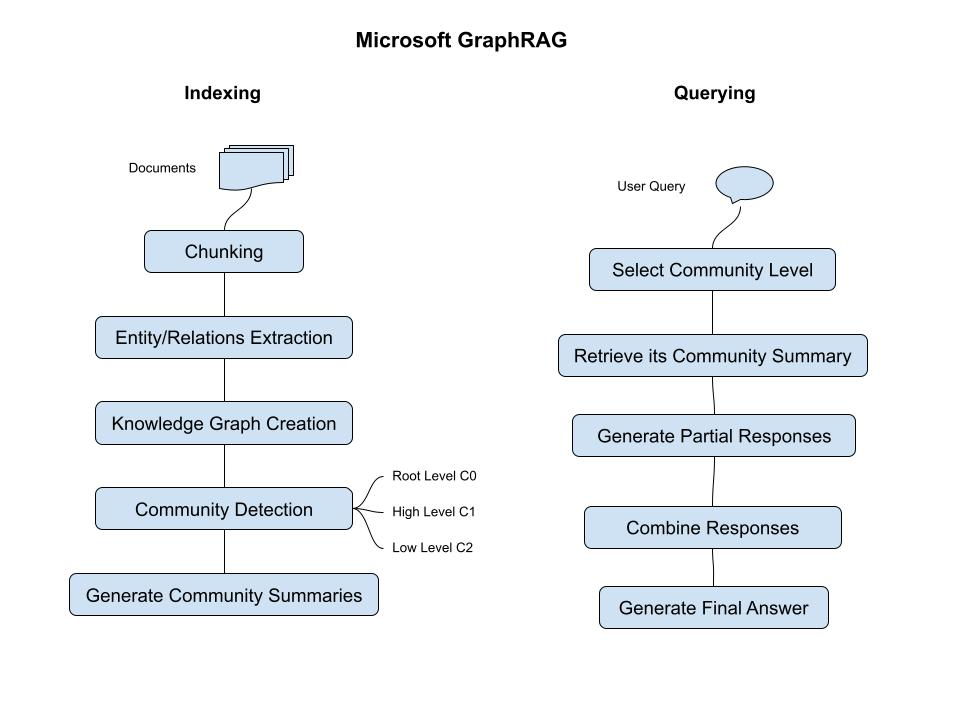
\includegraphics[width=\linewidth,keepaspectratio]{graphrag_ms}
	\end{center}
	
\end{frame}

%%%%%%%%%%%%%%%%%%%%%%%%%%%%%%%%%%%%%%%%%%%%%%%%%%%%%%%%%%%
\begin{frame}[fragile]\frametitle{Indexing Phase in GraphRAG}
  \begin{itemize}
    \item Chunk documents and extract entities and relationships.
    \item Build a knowledge graph from this information.
    \item Detect communities of closely related entities.
    \item Generate summaries at multiple community levels.
  \end{itemize}
\end{frame}

% %%%%%%%%%%%%%%%%%%%%%%%%%%%%%%%%%%%%%%%%%%%%%%%%%%%%%%%%%%%
% \begin{frame}[fragile]\frametitle{Summary Hierarchies}

	% \begin{center}
	% 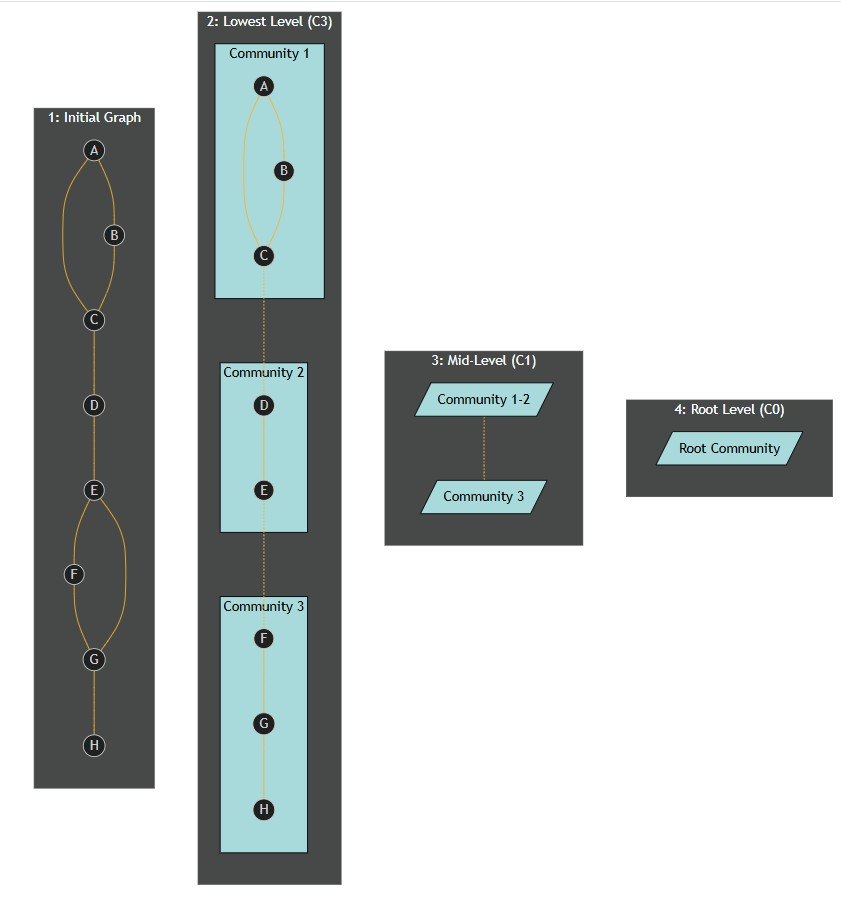
\includegraphics[width=0.6\linewidth,keepaspectratio]{graphrag_ms_3}
	% \end{center}
	
	% {\tiny (Ref: Graph RAG: Improving RAG with Knowledge Graphs: Prompt Engineering)}

	
% \end{frame}


%%%%%%%%%%%%%%%%%%%%%%%%%%%%%%%%%%%%%%%%%%%%%%%%%%%%%%%%%%%
\begin{frame}[fragile]\frametitle{Query Phase in GraphRAG}
  \begin{itemize}
    \item Select community level based on query detail needed.
    \item Retrieve relevant summaries from selected community.
    \item Combine responses from multiple communities if needed.
    \item Final answer is composed from merged summaries.
  \end{itemize}
\end{frame}



%%%%%%%%%%%%%%%%%%%%%%%%%%%%%%%%%%%%%%%%%%%%%%%%%%%%%%%%%%%
\begin{frame}[fragile]\frametitle{Setting Up GraphRAG Locally}
  \begin{itemize}
    \item Create and activate a Conda environment.
    \item Install the package:
  \end{itemize}
	
    \begin{lstlisting}[language=bash]
conda create -n GraphRag python=3.10
conda activate GraphRag
or
pip install graph-rag
    \end{lstlisting}
\end{frame}



%%%%%%%%%%%%%%%%%%%%%%%%%%%%%%%%%%%%%%%%%%%%%%%%%%%%%%%%%%%
\begin{frame}[fragile]\frametitle{Running the Indexing Process}
  \begin{itemize}
    \item Organize input data in a folder.
    \item Initialize configurations and set environment variables.
    \item Create index
    \item Requires API key and settings in `settings.yml`.
    \item Configure model (e.g., GPT-4o) and embedding model in `settings.yml`.
    \item Chunk size, overlap, and base API path are customizable.
    \item Prompt templates control how entities and summaries are extracted.	
  \end{itemize}

    \begin{lstlisting}[language=bash]
python -m graph_rag.index
    \end{lstlisting}  
\end{frame}

%%%%%%%%%%%%%%%%%%%%%%%%%%%%%%%%%%%%%%%%%%%%%%%%%%%%%%%%%%%
\begin{frame}[fragile]\frametitle{Querying with GraphRAG}
  \begin{itemize}
    \item Run queries
    \item Specify method: `global` for high-level themes, `local` for specific details.
    \item Responses cite sources and use graph structure to enhance relevance.
  \end{itemize}
    \begin{lstlisting}[language=bash]
python -m graph_rag.query
    \end{lstlisting}  
\end{frame}

% %%%%%%%%%%%%%%%%%%%%%%%%%%%%%%%%%%%%%%%%%%%%%%%%%%%%%%%%%%%%%%%%%%%%%%%%%%%%%%%%%%
% \begin{frame}[fragile]\frametitle{}
% \begin{center}
% {\Large End-to-End Flow with Neo4j}

% \end{center}
% \end{frame}

% %%%%%%%%%%%%%%%%%%%%%%%%%%%%%%%%%%%%%%%%%%%%%%%%%%%%%%%%%%%
% \begin{frame}[fragile]\frametitle{Setting Up GraphRAG}
	% \begin{itemize}
	% \item Install required dependencies
	% \item Configure environment variables
	% \end{itemize}
	% \begin{lstlisting}[language=bash]
	% pip install graphrag
	% pip install torch transformers neo4j

	% export NEO4J_URI="bolt://localhost:7687"
	% export NEO4J_USERNAME="neo4j"
	% export NEO4J_PASSWORD="password"
	% export OPENAI_API_KEY="your-key-here"
	% \end{lstlisting}
% \end{frame}

% %%%%%%%%%%%%%%%%%%%%%%%%%%%%%%%%%%%%%%%%%%%%%%%%%%%%%%%%%%%
% \begin{frame}[fragile]\frametitle{Document Ingestion Pipeline}
% Convert documents into graph-compatible format

	% \begin{lstlisting}[language=python]
	% from graphrag import DocumentProcessor

	% processor = DocumentProcessor()
	% documents = processor.load_documents("path/to/docs")
	% chunks = processor.chunk_documents(documents)
	% entities = processor.extract_entities(chunks)
	% relations = processor.extract_relations(chunks, entities)
	% \end{lstlisting}
% \end{frame}

% %%%%%%%%%%%%%%%%%%%%%%%%%%%%%%%%%%%%%%%%%%%%%%%%%%%%%%%%%%%
% \begin{frame}[fragile]\frametitle{Building the Knowledge Graph}
% Populate Neo4j with extracted entities and relationships

	% \begin{lstlisting}[language=python]
	% from graphrag import GraphBuilder

	% graph_builder = GraphBuilder(uri, username, password)
	% graph_builder.clear_database()  # Optional
	% graph_builder.create_schema()
	% graph_builder.add_entities(entities)
	% graph_builder.add_relationships(relations)
	% \end{lstlisting}
% \end{frame}

% %%%%%%%%%%%%%%%%%%%%%%%%%%%%%%%%%%%%%%%%%%%%%%%%%%%%%%%%%%%
% \begin{frame}[fragile]\frametitle{Knowledge Graph Embeddings}
% Generate embeddings for efficient graph retrieval

	% \begin{lstlisting}[language=python]
	% from graphrag import GraphEmbedder

	% embedder = GraphEmbedder(model="sentence-transformers/all-MiniLM-L6-v2")
	% embedder.generate_node_embeddings(graph_db)
	% embedder.generate_subgraph_embeddings(graph_db)
	% embedder.save_embeddings("embeddings.pkl")
	% \end{lstlisting}
% \end{frame}

% %%%%%%%%%%%%%%%%%%%%%%%%%%%%%%%%%%%%%%%%%%%%%%%%%%%%%%%%%%%
% \begin{frame}[fragile]\frametitle{Query Translation}
% Convert natural language queries to graph queries

	% \begin{lstlisting}[language=python]
	% from graphrag import QueryTranslator

	% translator = QueryTranslator(llm="gpt-4")
	% query = "Who funded the Manhattan Project?"
	% cypher_query = translator.to_cypher(query)
	% print(cypher_query)
	% # MATCH (p:Project {name: 'Manhattan Project'})-
	% # [:FUNDED_BY]->(f) RETURN f.name
	% \end{lstlisting}
% \end{frame}

% %%%%%%%%%%%%%%%%%%%%%%%%%%%%%%%%%%%%%%%%%%%%%%%%%%%%%%%%%%%
% \begin{frame}[fragile]\frametitle{Graph Retrieval Strategies}
	% \begin{itemize}
	% \item Multiple retrieval strategies for different query types
	% \item Direct query execution for structured data retrieval
	% \item Semantic search for similarity-based retrieval	
	% \end{itemize}
	% \begin{lstlisting}[language=python]
	% results = graph_db.execute_query(cypher_query)


	% from graphrag import SemanticGraphRetriever

	% retriever = SemanticGraphRetriever(embeddings)
	% relevant_nodes = retriever.retrieve(query, top_k=5)
	% \end{lstlisting}
% \end{frame}

% %%%%%%%%%%%%%%%%%%%%%%%%%%%%%%%%%%%%%%%%%%%%%%%%%%%%%%%%%%%
% \begin{frame}[fragile]\frametitle{Path-based Retrieval}
% Extract logical paths between relevant entities

	% \begin{lstlisting}[language=python]
	% from graphrag import PathRetriever

	% path_retriever = PathRetriever(graph_db)
	% paths = path_retriever.find_paths(
		% start_node="Albert Einstein", 
		% end_node="Manhattan Project",
		% max_length=3
	% )
	% \end{lstlisting}
% \end{frame}

% %%%%%%%%%%%%%%%%%%%%%%%%%%%%%%%%%%%%%%%%%%%%%%%%%%%%%%%%%%%
% \begin{frame}[fragile]\frametitle{Subgraph Extraction}
% Extract contextual subgraphs for complex queries

	% \begin{lstlisting}[language=python]
	% from graphrag import SubgraphExtractor

	% extractor = SubgraphExtractor(graph_db)
	% subgraph = extractor.extract_neighborhood(
		% seed_nodes=relevant_nodes, 
		% depth=2
	% )
	% \end{lstlisting}
% \end{frame}

% %%%%%%%%%%%%%%%%%%%%%%%%%%%%%%%%%%%%%%%%%%%%%%%%%%%%%%%%%%%
% \begin{frame}[fragile]\frametitle{Graph Reasoning}
% Apply graph algorithms to infer additional information

	% \begin{lstlisting}[language=python]
	% from graphrag import GraphReasoner

	% reasoner = GraphReasoner(graph_db)
	% inferences = reasoner.infer_relations(subgraph)
	% enhanced_graph = reasoner.enhance_subgraph(
		% subgraph, 
		% inferences
	% )
	% \end{lstlisting}
% \end{frame}

% %%%%%%%%%%%%%%%%%%%%%%%%%%%%%%%%%%%%%%%%%%%%%%%%%%%%%%%%%%%
% \begin{frame}[fragile]\frametitle{Response Generation}
% Generate responses using retrieved subgraphs

	% \begin{lstlisting}[language=python]
	% from graphrag import GraphRAGGenerator

	% generator = GraphRAGGenerator(
		% llm="gpt-4",
		% prompt_template="Based on the graph: {graph_context}\n\nQuestion: {query}\n\nAnswer:"
	% )

	% response = generator.generate(
		% query=query,
		% graph_context=enhanced_graph.to_text()
	% )
	% print(response)
	% \end{lstlisting}
% \end{frame}

% %%%%%%%%%%%%%%%%%%%%%%%%%%%%%%%%%%%%%%%%%%%%%%%%%%%%%%%%%%%
% \begin{frame}[fragile]\frametitle{End-to-End GraphRAG Pipeline}
% Complete pipeline from query to response

	% \begin{lstlisting}[language=python]
	% from graphrag import GraphRAGPipeline

	% pipeline = GraphRAGPipeline(
		% graph_db=graph_db,
		% retriever=retriever,
		% reasoner=reasoner,
		% generator=generator
	% )

	% answer = pipeline.run(query="What was Einstein's role in the Manhattan Project?")
	% print(answer)
	% \end{lstlisting}
% \end{frame}

% %%%%%%%%%%%%%%%%%%%%%%%%%%%%%%%%%%%%%%%%%%%%%%%%%%%%%%%%%%%
% \begin{frame}[fragile]\frametitle{Advanced Features: Query Decomposition}
% Break complex queries into simpler sub-queries

	% \begin{lstlisting}[language=python]
	% from graphrag import QueryDecomposer

	% decomposer = QueryDecomposer(llm="gpt-4")
	% complex_query = "How did Einstein's theories influence nuclear weapons development?"
	% sub_queries = decomposer.decompose(complex_query)
	% # ['What theories did Einstein develop?',
	% #  'How do these theories relate to nuclear physics?',
	% #  'How were these principles applied in weapons development?']
	% \end{lstlisting}
% \end{frame}

% %%%%%%%%%%%%%%%%%%%%%%%%%%%%%%%%%%%%%%%%%%%%%%%%%%%%%%%%%%%
% \begin{frame}[fragile]\frametitle{Advanced Features: Graph Augmentation}
% Dynamically enhance graph with new information

	% \begin{lstlisting}[language=python]
	% from graphrag import GraphAugmenter

	% augmenter = GraphAugmenter(
		% graph_db=graph_db,
		% llm="gpt-4"
	% )

	% new_entities = augmenter.extract_missing_entities(
		% query=query,
		% context=retrieved_text
	% )
	% graph_db.add_entities(new_entities)
	% \end{lstlisting}
% \end{frame}

% %%%%%%%%%%%%%%%%%%%%%%%%%%%%%%%%%%%%%%%%%%%%%%%%%%%%%%%%%%%
% \begin{frame}[fragile]\frametitle{Advanced Features: Explainability}
% Generate explanations for responses based on graph paths
	% \begin{lstlisting}[language=python]
	% from graphrag import ExplainableGraphRAG

	% explainable_rag = ExplainableGraphRAG(pipeline)
	% result = explainable_rag.generate(
		% query=query,
		% explain=True
	% )
	% print(f"Answer: {result['answer']}")
	% print(f"Explanation: {result['explanation']}")
	% print(f"Evidence paths: {result['evidence_paths']}")
	% \end{lstlisting}
% \end{frame}

% %%%%%%%%%%%%%%%%%%%%%%%%%%%%%%%%%%%%%%%%%%%%%%%%%%%%%%%%%%%
% \begin{frame}[fragile]\frametitle{Evaluation \& Benchmarking}
% Evaluate GraphRAG performance against standard benchmarks

	% \begin{lstlisting}[language=python]
	% from graphrag.evaluation import Evaluator

	% evaluator = Evaluator(
		% pipeline=pipeline,
		% metrics=["accuracy", "relevance", "faithfulness"]
	% )

	% results = evaluator.evaluate(
		% benchmark_dataset="path/to/questions.json"
	% )
	% print(f"Accuracy: {results['accuracy']}")
	% print(f"Relevance: {results['relevance']}")
	% \end{lstlisting}
% \end{frame}

%%%%%%%%%%%%%%%%%%%%%%%%%%%%%%%%%%%%%%%%%%%%%%%%%%%%%%%%%%%%%%%%%%%%%%%%%%%%%%%%%%
\begin{frame}[fragile]\frametitle{}
\begin{center}
{\Large Conclusions}

\end{center}
\end{frame}

%%%%%%%%%%%%%%%%%%%%%%%%%%%%%%%%%%%%%%%%%%%%%%%%%%%%%%%%%%%
\begin{frame}[fragile]\frametitle{GraphRAG: Evolution of Knowledge Graphs}
    \begin{itemize}
        \item Earlier, KGs were built using statistical and NLP techniques.
        \item GraphRAG scales efficiently by using LLMs for entity extraction.
        \item Entities in KG are nodes, linked by edges encoding relationships.
    \end{itemize}
\end{frame}

%%%%%%%%%%%%%%%%%%%%%%%%%%%%%%%%%%%%%%%%%%%%%%%%%%%%%%%%%%%
\begin{frame}[fragile]\frametitle{Key Features of GraphRAG}
    \begin{itemize}
        \item Maintains hierarchical communities preserving local and global insights.
        \item Ensures source traceability down to the node level for citations.
        \item Aggregates information from multiple sources, reducing bias.
        \item Focuses on meaningful nodes, filtering out irrelevant information.
    \end{itemize}
\end{frame}

%%%%%%%%%%%%%%%%%%%%%%%%%%%%%%%%%%%%%%%%%%%%%%%%%%%%%%%%%%%
\begin{frame}[fragile]\frametitle{Advantages of Knowledge Graphs}
    \begin{itemize}
        \item Connects information from multiple sources for deeper insights.
        \item Boosts retrieval accuracy and enables multi-hop reasoning.
        \item Enhances LLM responses by integrating structured relationships.
    \end{itemize}
\end{frame}

%%%%%%%%%%%%%%%%%%%%%%%%%%%%%%%%%%%%%%%%%%%%%%%%%%%%%%%%%%%
\begin{frame}[fragile]\frametitle{GraphRAG Cost Considerations}
  \begin{itemize}
    \item GraphRAG can be expensive—570 LLM requests vs. 25 embeddings.
    \item Over 1 million tokens processed cost around \$7 (using GPT-4).
    \item Cost increases with corpus size and LLM choice.
  \end{itemize}
\end{frame}

%%%%%%%%%%%%%%%%%%%%%%%%%%%%%%%%%%%%%%%%%%%%%%%%%%%%%%%%%%%
\begin{frame}[fragile]\frametitle{Alternatives and Ecosystem}
  \begin{itemize}
    \item Other GraphRAG implementations:
    \item \textbf{LlamaIndex} - Graph Query Engine.
    \item \textbf{Neo4j} - Native GraphRAG integration.
    \item Each offers different trade-offs in performance and cost.
  \end{itemize}
\end{frame}

%%%%%%%%%%%%%%%%%%%%%%%%%%%%%%%%%%%%%%%%%%%%%%%%%%%%%%%%%%%
\begin{frame}[fragile]\frametitle{Case Studies \& Applications}
	\begin{itemize}
	\item Enterprise knowledge management
	\item Scientific literature analysis
	\item Customer support and troubleshooting
	\item Regulatory compliance and legal research
	\item Healthcare and biomedical information systems
	\item Financial analysis and risk assessment
	\end{itemize}

\end{frame}





% %%%%%%%%%%%%%%%%%%%%%%%%%%%%%%%%%%%%%%%%%%%%%%%%%%%%%%%%%%%
% \begin{frame}[fragile]\frametitle{Traditional RAG Overview}
  % \begin{itemize}
    % \item Converts documents into vector embeddings via chunking.
    % \item Stores chunks in a vector database.
    % \item At query time: compute query embedding, retrieve similar chunks.
    % \item Combines query + retrieved chunks to generate final answer.
  % \end{itemize}
% \end{frame}

% %%%%%%%%%%%%%%%%%%%%%%%%%%%%%%%%%%%%%%%%%%%%%%%%%%%%%%%%%%%
% \begin{frame}[fragile]\frametitle{Limitations of Traditional RAG}
  % \begin{itemize}
    % \item Lacks holistic understanding of entire document set.
    % \item Retrieval efficiency drops as data size increases.
    % \item Complex integration of external knowledge sources.
  % \end{itemize}
% \end{frame}

% %%%%%%%%%%%%%%%%%%%%%%%%%%%%%%%%%%%%%%%%%%%%%%%%%%%%%%%%%%%
% \begin{frame}[fragile]\frametitle{GraphRAG: Key Concepts}
	% \begin{itemize}
	% \item Knowledge Graph (KG): Structured representation of entities and relationships
	% \item Graph Retrieval: Finding relevant graph sections for a given query
	% \item Graph Reasoning: Using graph structure to enhance LLM reasoning
	% \item Graph Augmentation: Dynamically enhancing the graph with new information
	% \item End-to-end pipeline combining these components with LLM generation
	% \end{itemize}
% \end{frame}

% %%%%%%%%%%%%%%%%%%%%%%%%%%%%%%%%%%%%%%%%%%%%%%%%%%%%%%%%%%%
% \begin{frame}[fragile]\frametitle{GraphRAG Architecture}
	% \begin{itemize}
	% \item Document Ingestion: Converting unstructured documents to graph format
	% \item Graph Store: Neo4j or other graph databases for storing knowledge
	% \item Embedding Engine: Creating vector representations of graph elements
	% \item Query Processing: Converting natural language to graph queries
	% \item Response Generation: Using retrieved subgraphs to augment LLM responses
	% \end{itemize}
% \end{frame}


% %%%%%%%%%%%%%%%%%%%%%%%%%%%%%%%%%%%%%%%%%%%%%%%%%%%%%%%%%%%
% \begin{frame}[fragile]\frametitle{Resources \& Next Steps}
	% \begin{itemize}
	% \item GitHub Repository: https://github.com/microsoft/graphrag
	% \item Documentation: Full API reference and tutorials
	% \item Examples: Comprehensive example notebooks
	% \item Community: GitHub discussions and issue tracker
	% \item Extensions: Integration with other frameworks
	% \item Updates: Regular releases with new features
	% \end{itemize}
% \end{frame}

% %%%%%%%%%%%%%%%%%%%%%%%%%%%%%%%%%%%%%%%%%%%%%%%%%%%%%%%%%%%
% \begin{frame}[fragile]\frametitle{Microsoft GraphRAG Workflow}

	
	% \begin{center}
	% 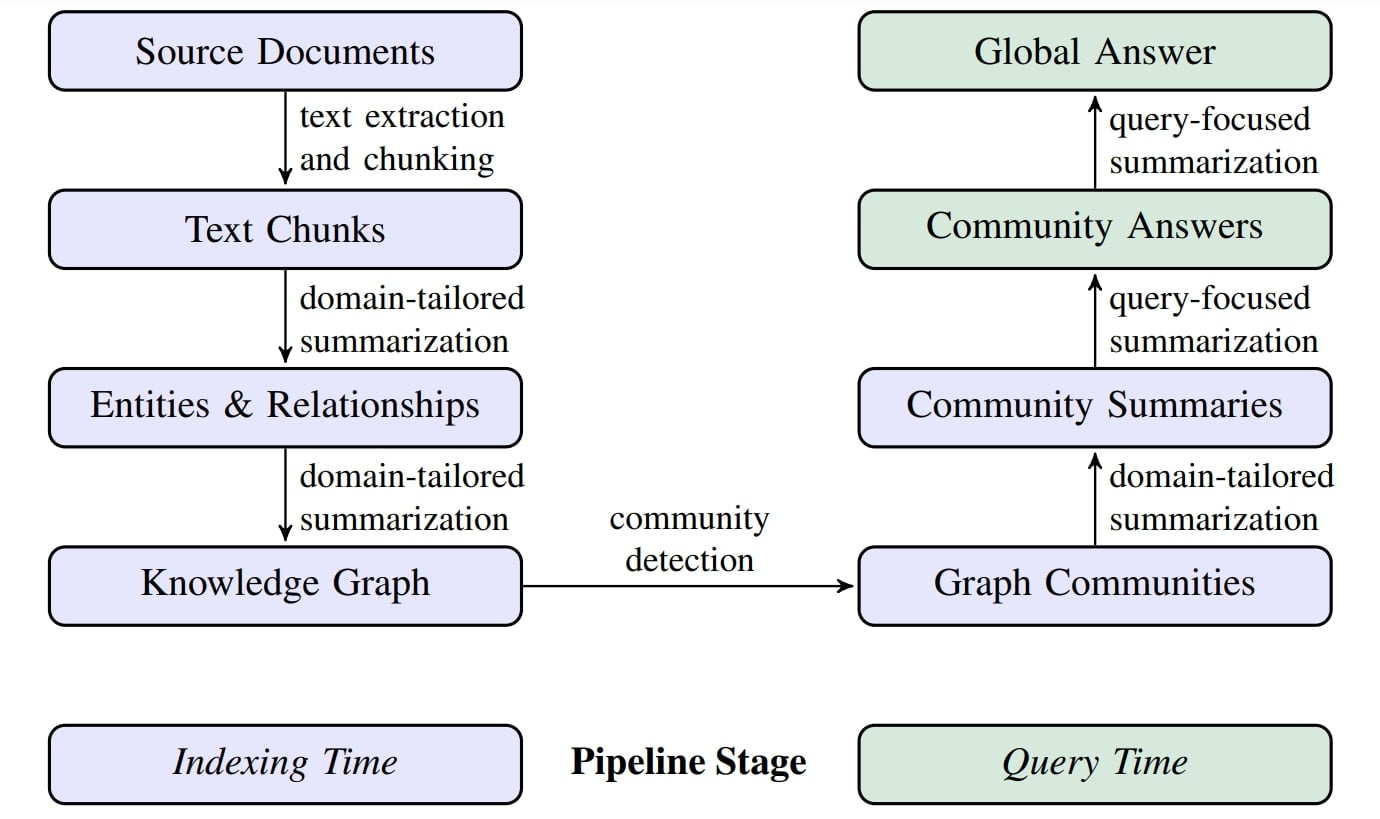
\includegraphics[width=\linewidth,keepaspectratio]{graphrag18}
	
	% {\tiny (Ref: GraphRAG: The Practical Guide for Cost-Effective Document Analysis with Knowledge Graphs -Jaykumaran)}
	% \end{center}	
% \end{frame}

% %%%%%%%%%%%%%%%%%%%%%%%%%%%%%%%%%%%%%%%%%%%%%%%%%%%%%%%%%%%
% \begin{frame}[fragile]\frametitle{Indexing Phase Overview}
    % \begin{itemize}
        % \item Two-stage process: Generate Knowledge Graph (KG) and Community Clustering.
        % \item Extract entities and relationships, construct KG.
        % \item Partition KG into semantically related clusters.
        % \item Generate community summaries for optimized retrieval.
    % \end{itemize}
% \end{frame}

% %%%%%%%%%%%%%%%%%%%%%%%%%%%%%%%%%%%%%%%%%%%%%%%%%%%%%%%%%%%
% \begin{frame}[fragile]\frametitle{Step 1: Segment Documents into Chunks}
    % \begin{itemize}
        % \item Large text split into smaller chunks for LLM processing.
        % \item Small chunks retain details but increase API cost.
        % \item Larger chunks reduce cost but may omit key data.
        % \item Self-reflection in prompts improves extraction accuracy.
    % \end{itemize}
% \end{frame}

% %%%%%%%%%%%%%%%%%%%%%%%%%%%%%%%%%%%%%%%%%%%%%%%%%%%%%%%%%%%
% \begin{frame}[fragile]\frametitle{Step 2: Extract Entities and Relationships}
    % \begin{itemize}
        % \item LLM extracts entities, relationships, and descriptions.
        % \item Entities assigned unique IDs for traceability.
        % \item Pronouns and ambiguities resolved.
    % \end{itemize}

    % \begin{lstlisting}
    % {
      % "nodes": [
        % {"id": "n0", "entity_type": "PATIENT", "name": "71-YEAR-OLD GENTLEMEN"},
        % {"id": "n1", "entity_type": "DIAGNOSIS", "name": "PERIPHERAL VASCULAR DISEASE"}
      % ],
      % "edges": [
        % {"id": "e0", "source": "n0", "target": "n1", "description": "Patient has history of this condition"}
      % ]
    % }
    % \end{lstlisting}
% \end{frame}

% %%%%%%%%%%%%%%%%%%%%%%%%%%%%%%%%%%%%%%%%%%%%%%%%%%%%%%%%%%%
% \begin{frame}[fragile]\frametitle{Step 2: Extract Entities and Relationships}

    % \begin{lstlisting}
% **-Goal-**
% Given a text document that is potentially relevant to this activity and a list of entity types, identify all entities of those types from the text and all relationships among the identified entities.
 
% -Steps-
% 1. Identify all entities. For each identified entity, extract the following information:
% - entity_name: Name of the entity, capitalized
% - entity_type: One of the following types: [{entity_types}]
% - entity_description: Comprehensive description of the entity's 

% 2. From the entities identified in step 1, identify all pairs of (source_entity, target_entity) that are *clearly related to each other.
 
% For each pair of related entities, extract the following information:
% - source_entity: name of the source entity, as identified in step 1
% - target_entity: name of the target entity, as identified in step 1
% - relationship_description: explanation as to why you think the source entity and the target entity are related to each other
% - relationship_strength: a numeric score indicating strength of the relationship between the source entity and target entity
    % \end{lstlisting}
% \end{frame}


% %%%%%%%%%%%%%%%%%%%%%%%%%%%%%%%%%%%%%%%%%%%%%%%%%%%%%%%%%%%
% \begin{frame}[fragile]\frametitle{Step 2: Extract Entities and Relationships}

    % \begin{lstlisting}
% # Entities: 
% {
  % "nodes": [
    % {
      % "id": "n0",
      % "entity_type": "PATIENT",
      % "description": "A male patient aged 71 with several medical conditions",
      % "source_id": "n0",
      % "name": "71-YEAR-OLD GENTLEMEN"
    % },
    % {
      % "id": "n1",
      % "entity_type": "DIAGNOSIS",
      % "description": "Condition treated with right leg angioplasty\nPeripheral vascular disease (PVD) is a circulatory condition characterized by narrowed or blocked arteries outside of the heart and brain, leading to reduced blood flow, particularly to limbs. Patients with PVD may have undergone procedures like angioplasty in affected areas to improve circulation. Treatment generally involves medications such as Plavix and aspirin, as well as surgical interventions based on individual assessments.",
      % "source_id": "n1",
      % "name": "PERIPHERAL VASCULAR DISEASE"
    % },
    % \end{lstlisting}
% \end{frame}


% %%%%%%%%%%%%%%%%%%%%%%%%%%%%%%%%%%%%%%%%%%%%%%%%%%%%%%%%%%%
% \begin{frame}[fragile]\frametitle{Step 2: Extract Entities and Relationships}

    % \begin{lstlisting}
% # Relations
 % "edges": [
    % {
      % "id": e0,
      % "source": "n0",
      % "target": "n1",
      % "description": "The patient has a medical history of this condition",
    % },
    % {
      % "id": e1,
      % "source": "n0",
      % "target": "n2",
      % "description": "Chronic Obstructive Pulmonary Disease is part of his health profile",
    % },
    % \end{lstlisting}
% \end{frame}


% %%%%%%%%%%%%%%%%%%%%%%%%%%%%%%%%%%%%%%%%%%%%%%%%%%%%%%%%%%%
% \begin{frame}[fragile]\frametitle{Step 3: Construct Knowledge Graph}
    % \begin{itemize}
        % \item Entities and relationships aggregated into a unified KG.
        % \item Duplicates merged for efficiency.
    % \end{itemize}
% \end{frame}

% %%%%%%%%%%%%%%%%%%%%%%%%%%%%%%%%%%%%%%%%%%%%%%%%%%%%%%%%%%%
% \begin{frame}[fragile]\frametitle{Step 4: Graph Partitioning into Communities}
    % \begin{itemize}
        % \item Leiden algorithm partitions KG into clusters.
        % \item Hierarchical approach ensures fine granularity.
        % \item Nodes belong to only one community.
        % \item Dynamic community selection at multiple levels.
    % \end{itemize}
	
	% \begin{center}
	% 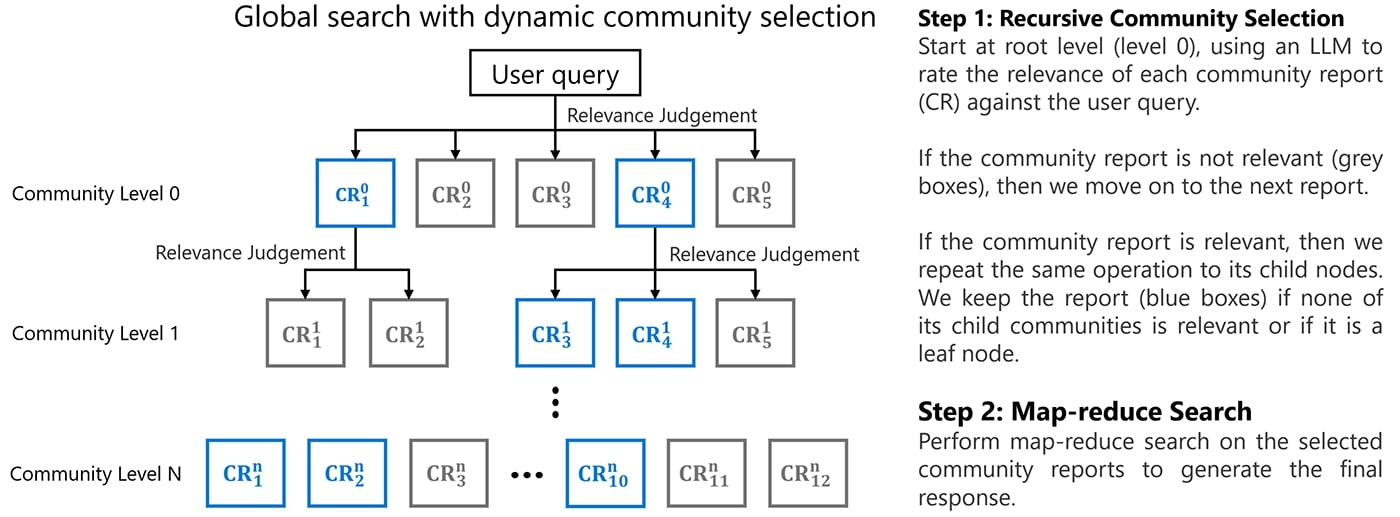
\includegraphics[width=\linewidth,keepaspectratio]{graphrag19}
	
	% {\tiny (Ref: GraphRAG: The Practical Guide for Cost-Effective Document Analysis with Knowledge Graphs -Jaykumaran)}
	% \end{center}	
% \end{frame}

% %%%%%%%%%%%%%%%%%%%%%%%%%%%%%%%%%%%%%%%%%%%%%%%%%%%%%%%%%%%
% \begin{frame}[fragile]\frametitle{Step 5: Community Summarization}

    % \begin{lstlisting}[language=markdown]
% # **Goal**
% Write a comprehensive report of a community, given a list of entities that belong to the community as well as their relationships and optional associated claims. The report will be used to inform decision-makers about information associated with the community and their potential impact. The content of this report includes an overview of the community's key entities, their legal compliance, technical capabilities, reputation, and noteworthy claims.

    % \end{lstlisting}	
% \end{frame}

% %%%%%%%%%%%%%%%%%%%%%%%%%%%%%%%%%%%%%%%%%%%%%%%%%%%%%%%%%%%
% \begin{frame}[fragile]\frametitle{Step 5: Community Summarization}

    % \begin{lstlisting}[language=markdown]
% # Report Structure
% The report should include the following sections:
 
% - TITLE: community's name that represents its key entities 
% - SUMMARY: An executive summary of the community's overall structure,
% - IMPACT SEVERITY RATING: a float score between 0-10 that represents the severity of IMPACT posed by entities within the community. 
% - RATING EXPLANATION: Give a single sentence explanation of the IMPACT severity rating.
% - DETAILED FINDINGS: A list of 5-10 key insights about the community.
    % \end{lstlisting}	
% \end{frame}

% %%%%%%%%%%%%%%%%%%%%%%%%%%%%%%%%%%%%%%%%%%%%%%%%%%%%%%%%%%%
% \begin{frame}[fragile]\frametitle{Querying Phase Overview}
    % \begin{itemize}
        % \item Identifies key entities and relationships in queries.
        % \item Retrieves relevant community summaries instead of entire KG.
    % \end{itemize}
% \end{frame}

% %%%%%%%%%%%%%%%%%%%%%%%%%%%%%%%%%%%%%%%%%%%%%%%%%%%%%%%%%%%
% \begin{frame}[fragile]\frametitle{Query Focused Summarization (QFS)}
    % \begin{itemize}
        % \item Identifies patterns and correlations from queries.
        % \item Matches against community summaries.
        % \item Optimized retrieval ensures efficient responses.
    % \end{itemize}
% \end{frame}

% %%%%%%%%%%%%%%%%%%%%%%%%%%%%%%%%%%%%%%%%%%%%%%%%%%%%%%%%%%%
% \begin{frame}[fragile]\frametitle{Map Reduce Approach}
    % \begin{itemize}
        % \item \textbf{Map Phase}: Generates multiple partial responses with importance scores.
        % \item \textbf{Reduce Phase}: Sorts and merges top-scoring responses into a global answer.
        % \item Efficiently filters search space while maintaining accuracy.
    % \end{itemize}
	
	% \begin{center}
	% 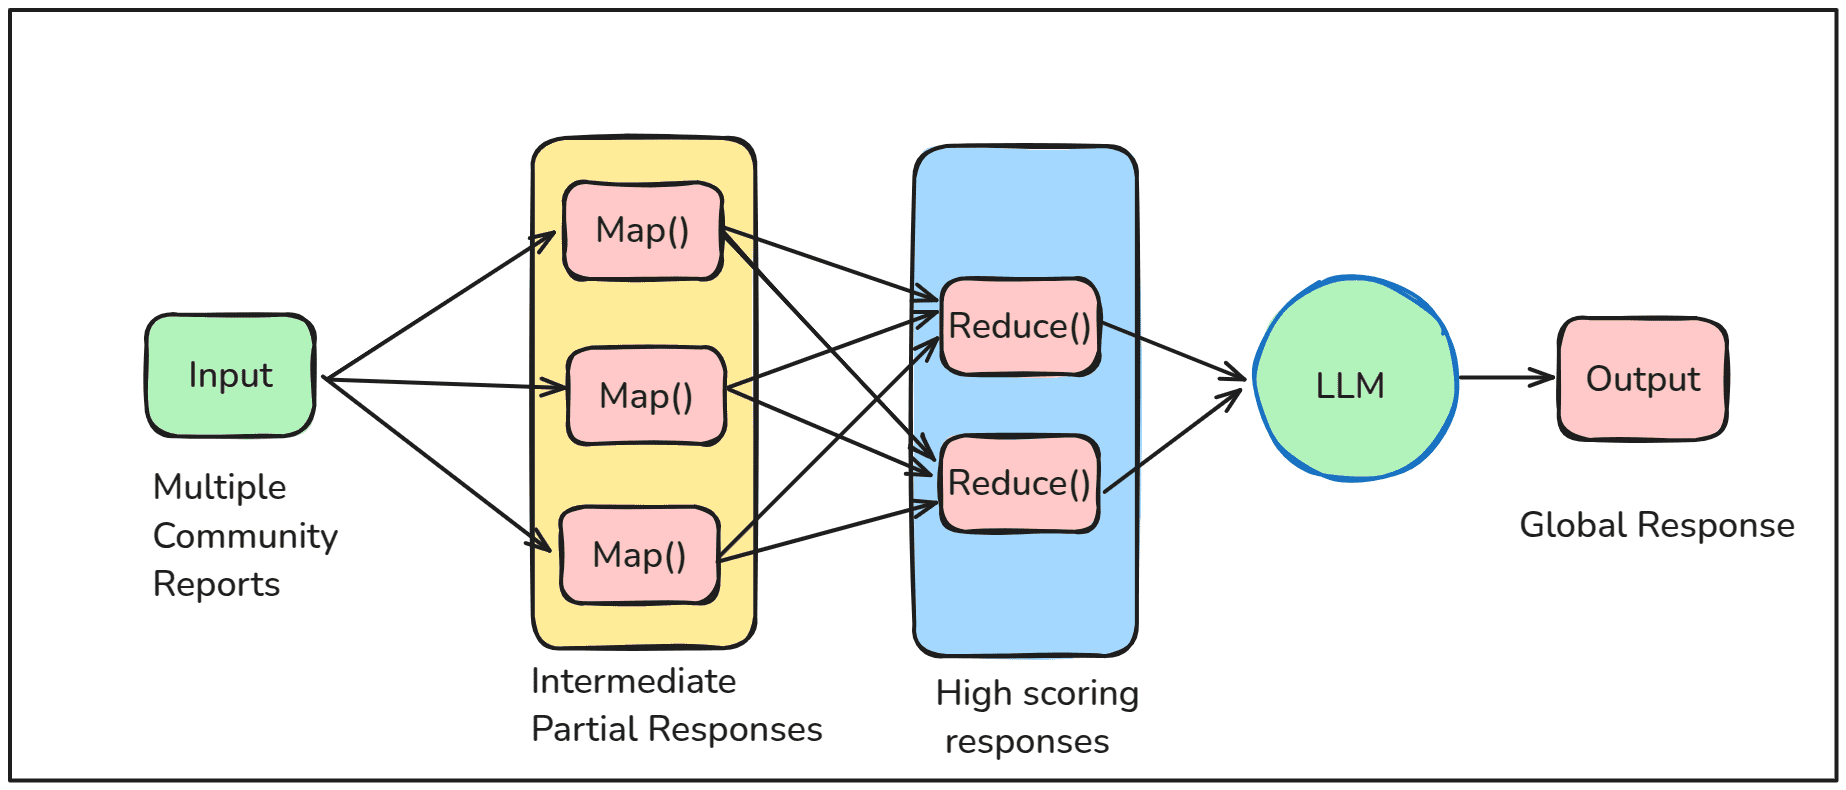
\includegraphics[width=\linewidth,keepaspectratio]{graphrag20}
	
	% {\tiny (Ref: GraphRAG: The Practical Guide for Cost-Effective Document Analysis with Knowledge Graphs -Jaykumaran)}
	% \end{center}		
% \end{frame}



% %%%%%%%%%%%%%%%%%%%%%%%%%%%%%%%%%%%%%%%%%%%%%%%%%%%%%%%%%%%
% \begin{frame}[fragile]\frametitle{Benchmarks and Evaluation Metrics}
    % \begin{itemize}
        % \item Traditional RAGAS metrics are inadequate for sensemaking queries.
        % \item LLM judges responses based on:
        % \begin{itemize}
            % \item \textbf{Comprehensiveness}: Covers all aspects of the query.
            % \item \textbf{Diversity}: Provides varied perspectives and insights.
            % \item \textbf{Empowerment}: Aids decision-making without false assumptions.
            % \item \textbf{Directness}: Clear, concise, and to the point.
        % \end{itemize}
        % \item GraphRAG excels in comprehensiveness and diversity.
        % \item Naive RAG is better at generating direct answers.
    % \end{itemize}
% \end{frame}

% %%%%%%%%%%%%%%%%%%%%%%%%%%%%%%%%%%%%%%%%%%%%%%%%%%%%%%%%%%%
% \begin{frame}[fragile]\frametitle{Shortcomings of Microsoft GraphRAG}
    % \begin{itemize}
        % \item Multiple LLM API calls make it slow, inefficient, and costly.
        % \item No de-duplication step, resulting in a noisy graph index.
        % \item Upserting new data requires reconstructing the entire KG, making it impractical for production.
    % \end{itemize}
% \end{frame}


% %%%%%%%%%%%%%%%%%%%%%%%%%%%%%%%%%%%%%%%%%%%%%%%%%%%%%%%%%%%
% \begin{frame}[fragile]\frametitle{GraphRAG Alternatives and Improvements}
    % \begin{itemize}
        % \item Graph-based RAG is not new; earlier versions by NebulaGraph, Langchain, LlamaIndex, Neo4j.
        % \item Microsoft's approach became widely accepted but has limitations.
        % \item Led to new variants focusing on efficiency and accuracy.
    % \end{itemize}
% \end{frame}

% %%%%%%%%%%%%%%%%%%%%%%%%%%%%%%%%%%%%%%%%%%%%%%%%%%%%%%%%%%%
% \begin{frame}[fragile]\frametitle{GraphRAG Variants}
    % \begin{itemize}
        % \item \textbf{Nano-GraphRAG}: Introduced lighter, faster versions.
        % \item \textbf{Top-k Selection}: Unlike map-reduce, it selects only top-k communities for efficiency.
        % \item Derived versions: LightRAG, MedGraphRAG, FastGraphRAG.
        % \item MedGraphRAG is challenging to adapt to OpenAI endpoints.
    % \end{itemize}
% \end{frame}



% %%%%%%%%%%%%%%%%%%%%%%%%%%%%%%%%%%%%%%%%%%%%%%%%%%%%%%%%%%%
% \begin{frame}[fragile]\frametitle{Challenges with Microsoft's GraphRAG}
    % \begin{itemize}
        % \item Too expensive and impractical for large-scale industrial use.
        % \item Most companies prefer standard vector databases.
        % \item Lack of widespread production adoption due to cost and complexity.
    % \end{itemize}
% \end{frame}



% %%%%%%%%%%%%%%%%%%%%%%%%%%%%%%%%%%%%%%%%%%%%%%%%%%%%%%%%%%%
% \begin{frame}[fragile]\frametitle{Text-To-Cypher/SPARQL Alternative}
    % \begin{itemize}
        % \item Effective alternative to Microsoft's GraphRAG.
        % \item Requires costly LLM calls for query generation.
        % \item Adds uncertainty due to prompt effectiveness and model performance.
        % \item Increases response time and implementation complexity.
    % \end{itemize}
% \end{frame}
